% ----------------------------------------------------------
% Seção Lógica - Principal
% ----------------------------------------------------------
\section{Lógica}
Segundo o dicionário online de Português Dicio\cite{dicio_logica}, a palavra lógica se refere a:
\begin{enumerate}
   \item Modo de raciocinar coerente que \underline{expressa uma relação de causa e consequência};
   \item Maneira coerente através da qual os \underline{fatos ou situações se encadeiam}. 
\end{enumerate}
 
\bigbreak
A palavra lógica expressa uma relação de causa e consequência ou fatos encadeados. Pode-se distinguir como essência dessas duas definições o movimento, a mudança, a transição. A palavra lógica, em sua essência, se encaixa perfeitamente na definição do NADA − NÃO SER.  A lógica NÃO SER é consonante com o NADA, pois se a lógica NÃO É ela também É seu contrário, ou seja, ilógica e imutável. Nessa dualidade, tem-se a existência fundamentada pela lógica que "nega a si", enquanto, por outro lado É ilógica, imutável e inexistente. A expressão "negação de si" refere-se à negação do SER - NÃO SER. 

A lógica está centrada na mudança e a mudança está centrada naquilo que NÃO É, uma vez que aquilo que É não pode deixar de SER. A mudança demanda que, em algum momento, algo DEIXE DE SER o que fora a se transformar. Em \citeonline{brasilescola_parmenides}, Parmênides  o filósofo da unidade e da identidade do SER, diz que a contínua mudança é a principal característica do não ser. Para Parmênides o SER é uno, eterno, não gerado e imutável.

A lógica SER ilógica não a impede de NÃO SER.  Na dualidade SER e NÃO SER, o SER limita e define o NÃO SER \textit{ad infinitum}. É possível se aproximar da definição do SER enumerando e definindo infinitamente tudo o que ele NÃO É.

\begin{figure}[H]
\caption{Analogia da lógica primordial}
\label{fig:primordial_logic_representation}
\centering
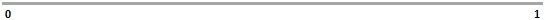
\includegraphics[scale=1]{sections/images/primordial_logic_representation.jpg}
\floatfoot{Reta utilizada para representar e validar o conceito da lógica primordial.}%\footnotemark}
\end{figure}
%\footnotetext{Fonte: note}

Com base na Figura \ref{fig:primordial_logic_representation} pode-se extrair as seguintes observações em relação aos pontos \textbf{0}, \textbf{1} e o \textbf{intervalo} entre eles:
\begin{description}
   \item[Ponto 1 - {[1,1]}] É ilógico, pois é a totalidade não fracionada da reta.
   \item[Ponto 0 - {[0,0]}] É ilógico, pois é um ponto nulo incapaz de negar a si, dado que toda lógica ou sub-lógica (fração lógica) deve se manter negando a si, dado que essa é a premissa básica da lógica. A lógica NÃO É em sua essência, primordialmente.
   \item[Intervalo - $\textbf{{[0,1[ x ]0,1]}}$] A lógica é possível apenas na representação das frações ou intervalos dos pontos \textbf{0} e \textbf{1}. Uma fração da reta nega ser a reta, pois é apenas uma parte dela. Os subintervalos são hábeis a negar a si infinitamente, garantindo a premissa primordial da lógica e suas sub-lógicas, negar a si. 
\end{description}

\begin{figure}[H]
\caption{Primeiro momento lógico}
\label{fig:first_logical_moment}
\centering

\includegraphics[scale=1]{sections/images/first_logical_moment.jpg}
\floatfoot{Reta fracionada em dois intervalos representando o primeiro momento lógico.}%\footnotemark}
\end{figure}
%\footnotetext{Fonte: note}

Na Figura \ref{fig:first_logical_moment} a união do traço à reta é a representação de uma divisão lógica, pois é da negação da lógica em SER que surgi esses dois intervalos lógicos ou duas sub-lógicas. O segmento em azul representa a negação da lógica em SER o todo ilógico nesse primeiro momento. As duas frações geradas pela negação lógica negam SER a reta, pois são apenas intervalos delas e são capazes de negar a si infinitamente, garantindo a premissa primordial da lógica NÃO SER. 

% ----------------------------------------------------------
% Subseção Expansão lógica
% ----------------------------------------------------------
\subsection{Expansão lógica}
A lógica primordial (negação de si) cria expansões lógicas infinitas. Uma expansão lógica é análoga a um universo. O primeiro momento lógico é o início de uma dessas expansões, porém existem infinitas possibilidades de negação do primeiro momento lógico, o que revela a possibilidade das infinitas expansões lógicas, pois o SER é imutável, portanto pode ser negado infinitamente. A negação do SER não transforma SER em NÃO SER, pois este é imutável. O NÃO SER é a pluralidade do imutável, singular e inexistente SER. 
	\begin{figure}[H]
	\caption{Momentos lógicos iniciais}
	\label{fig:third_logical_moment}
	\centering
	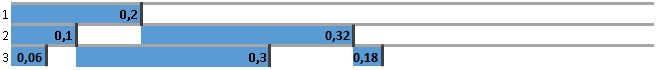
\includegraphics[scale=.85]{sections/images/third_logical_moment.jpg}
	\floatfoot{Exemplo dos três primeiros momentos de uma expansão.}%\footnotemark}
	\end{figure}
	%\footnotetext{Fonte: note}

Com base na Figura \ref{fig:third_logical_moment} pode-se extrair as seguintes observações em relação ao primeiro, segundo e terceiro momentos lógicos:
	\begin{description}
	   \item[Primeiro momento lógico] A negação da lógica primordial a si, a subdivide em duas unidades, que somadas são o todo ilógico. Apesar dessas partes terem proporções diferentes, elas exprimem as mesmas quantidades de pontos ou possibilidades de mudança, uma vez que são representações da lógica primordial, que \textit{ad infinitum}. A parte fracionada em azul representa a proporção da negação lógica em relação à sua unidade.
	   \item[Segundo momento lógico] É gerado pela negação das duas sub-lógicas primordiais, fracionadas no primeiro momento lógico. Na impossibilidade dessas frações lógicas do primeiro momento lógico continuar negando a si, faria com que elas fossem incapazes de negar suas unidades que formam o todo, ou seja, seriam incapazes de negar suas duas unidades e por consequência o todo que é formado precisamente por elas, o que faria da lógica apenas ilógica (SER), uma unicidade. As partes fracionadas em azul representam a proporção da negação lógica em relação às suas respectivas unidades.
	   \item[Terceiro momento lógico] Decorre da negação do segundo momento lógico, assim como o segundo momento lógico decorre da negação do primeiro e assim por diante.
	\end{description}

A cada negação ou subnegação da lógica primordial, seus novos valores são influenciados pelos valores adjacentes do momento lógico anterior. Na figura \ref{fig:imposition_of_binomial_expansion}, a lógica primordial nega a si gerando o primeiro momento lógico com o valor [0,2].  No segundo momento lógico, suas subdivisões estão contidas no limite imposto pelo valor do primeiro momento lógico. Os pontos do terceiro momento lógico, por exemplo, sofrem as imposições dos valores do segundo momento lógico que por sua vez sofrem a imposição do primeiro. Os valores de momentos lógicos descendentes sofrem imposições acumulativas dos valores dos momentos lógicos anteriores. À imposição de um valor em seus dois valores imediatamente descendentes denominou-se sincronismo lógico. Isso é o que pode ser visto no triângulo de pascal. Esse sincronismo irá levar à frequências de amostras cada vez maiores em intervalos centralizados cada vez menores, que serão vistos na próxima seção do teorema central do limite.
	\begin{figure}[H]
	\caption{Imposição da expansão lógica}
	\label{fig:imposition_of_binomial_expansion}
	\centering
	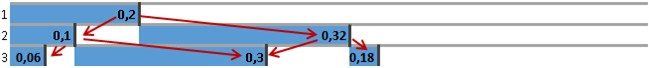
\includegraphics[scale=.85]{sections/images/imposition_of_binomial_expansion.jpg}
	\floatfoot{Imposição acumulativa aos momentos lógicos descendentes.}%\footnotemark}
	\end{figure}
	%\footnotetext{Fonte: note}

No triângulo de pascal, Figura \ref{fig:pascal_triangle}, cada número é os dois números acima mais próximos somados. Esse número representa quantos diferentes possíveis caminhos levam até ele. Por exemplo, o número [4], na Figura \ref{fig:pascal_triangle}, representa os quatro diferentes caminhos que levam até ele. Os coeficientes binômias encontrados no triangulo de Pascal representam apenas as quantidades de imposições sofridas por cada valor de um momento lógico. Um outro aspecto interessante do triângulo de pascal é a sequência de Fibonacci, Figura \ref{fig:pascal_triangle_fibonacci} \cite{mathisfun_pascal_triangle}.  
\enlargethispage{\baselineskip}
	\begin{figure}[H]
	\centering
		\begin{subfigure}[H]{0.47\linewidth}
		\centering
		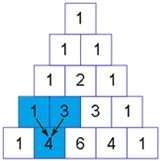
\includegraphics[width=.55\linewidth]{sections/images/pascal_triangle.jpg}
		\caption{}
		\label{fig:pascal_triangle}
		\end{subfigure}
	\hfill
		\begin{subfigure}[H]{0.47\linewidth}
		\centering
		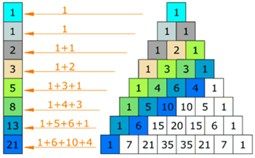
\includegraphics[width=.9\linewidth]{sections/images/pascal_triangle_fibonacci.jpg}
		\caption{}
		\label{fig:pascal_triangle_fibonacci}
		\end{subfigure}%
	\caption{Características do triângulo de Pascal}
	\floatfoot{Fonte: MathsIsFun, 2019. \protect\footnotemark}
	\end{figure}
	\footnotetext{\url{www.mathsisfun.com/pascals-triangle.html}}

O NÃO SER da lógica primordial é análogo a uma constante abstrata, ou seja, suas infinitas negações e subnegações transcendem o tempo. Todas essas infinitas negações acontecem no tempo zero. A incapacidade da lógica negar a si por um intervalo entre suas negações faria a lógica SER ilógica nesse intervalo, por menor que este seja, o que quebraria a premissa primordial da lógica, NÃO SER. A lógica é como um algoritmo composto de apenas uma constante auto executada, uma sequência simultânea. É a consciência que conduz a experiência do tempo, não pela criação da sequência de mudanças que é simultânea, mas sim pela ordem dessa sequência, que nada mais é que do que a observação da ordem das mudanças de cada momento lógico.

Algumas respostas podem ajudar a esclarecer o que é essa sequência simultânea:
	\begin{description}
	   \item[Todas as negações acontecem simultaneamente?] Sim, infinitas negações na ausência de tempo, ou tempo zero.
	   \item[Como ou porque essa simultaneidade acontece?] Acontecem em uma sequência de negações da lógica a si mesma, no tempo zero, onde em nenhum momento a lógica converte-se em SER, garantindo assim a premissa primordial da constante lógica, NÃO SER.
	   \item[O que é uma sequência simultânea?] É a negação da lógica a si (uma sequência) no tempo zero, ou seja, em nenhum momento a lógica passa a SER durante as infinitas negações (simultaneidade). Sequência simultânea é o sinônimo da constante lógica NÃO SER.
	\end{description}

Em outras palavras, é como uma constante abstrata com infinitos momentos lógicos e com infinitas expansões lógicas desses momentos. Ou pode-se pensar como uma reta e seus infinitos pontos onde cada ponto se conecta a todos os outros que lhes cabem formando infinitos momentos lógicos e infinitas expansões lógicas desses momentos.

% ----------------------------------------------------------
% Subseção Teorema central do limite
% ----------------------------------------------------------
\subsection{Teorema central do limite}
\lipsum[2]



% ----------------------------------------------------------
% Subseção Consciência
% ----------------------------------------------------------
\subsection{Consciência}
Um momento lógico pode ser formado por uma divisão (primeiro momento) ou por subdivisões lógicas (demais momentos).
	\begin{figure}[H]
	\caption{Intervalo lógico}
	\label{fig:consciousness_logical_moments}
	\centering
	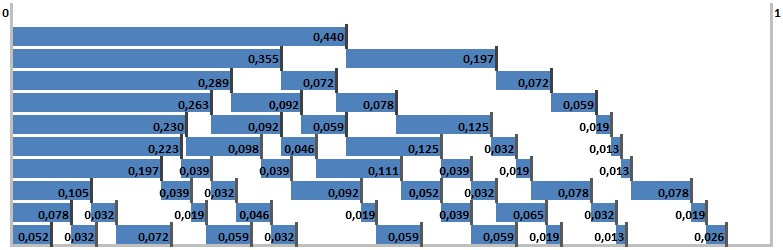
\includegraphics[scale=.7]{sections/images/consciousness_logical_moments.jpg}
	\floatfoot{Exemplo de um intervalo lógico com dez momentos lógicos.}%\footnotemark}
	\end{figure}
	%\footnotetext{Fonte: note}

A consciência são os momentos lógicos de uma expansão representados em suas unidades.
	\begin{figure}[H]
	\caption{Intervalo lógico consciente}
	\label{fig:consciousness}
	\centering
	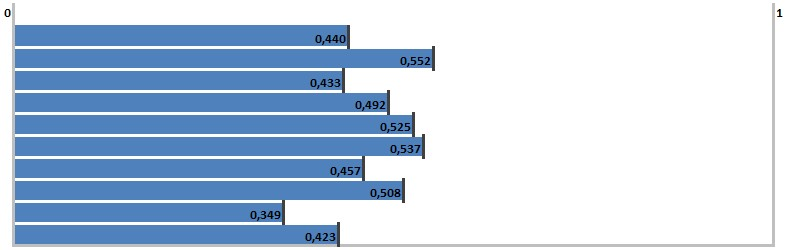
\includegraphics[scale=.7]{sections/images/consciousness.jpg}
	\floatfoot{Exemplo de um intervalo lógico consciente com dez unidades de momentos lógicos.}%\footnotemark}
	\end{figure}
	%\footnotetext{Fonte: note}

Pode ser observado na Tabela \ref{tab:10000_all} que a probabilidade de 99,99\% das amostras (Amostras do Range), que aumentam em quantidade a medida que crescem os momentos lógicos, tendem a estar cada vez mais ao centro do intervalo lógico, sendo que essa centralização tende ao infinito.
	\begin{figure}[H]
	\caption{Centralização de 99,99\% das amostras}
	\label{fig:centering_of_99_range}
	\centering
	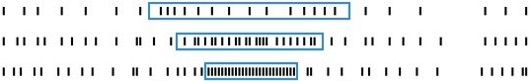
\includegraphics[scale=1]{sections/images/centering_of_99_range.jpg}
	\floatfoot{Tendência de centralização do range de 99,99\% das amostras.}%\footnotemark}
	\end{figure}
	%\footnotetext{Fonte: note}

A consciência tende à representação de um histograma da distribuição normal. Todos os aspectos listados abaixo são inerentes a abstração lógica chamada consciência.

\subsubsection{Infinito}
Um dos aspectos mais importantes que a negação do nada traz (negação de si), é o infinito, ou seja, em qualquer intervalo lógico cabe o infinito novamente. A lógica primordial que iniciou todo o intervalo lógico é a mesma encontrada em seus intervalos subsequentes. Isso fundamenta como uma lógica de alto nível como a subconsciência humana explica a lógica primordial, uma vez que não é preciso voltar ao primeiro momento lógico do intervalo para deduzi-lo, pois esse fenômeno é onipresente em todo o intervalo.

\subsubsection{Ondas}
Probabilisticamente a distribuição de novas amostras de uma população tendem a concentrar mais amostras sentido a mediana da população com frequências de amostras cada vez maiores neste sentido. Porém, a distribuição dessas amostras com frequências de crescimento uniformes é infinitesimal se comparado às possibilidades randômicas desse crescimento. Assim, a tendência de crescimento dessas frequências sentido a mediana somadas a baixíssima probabilidade (infinitesimal) desse crescimento ser uniforme, conduz a frequências no padrão de ondas.
	\begin{figure}[H]
	\caption{Padrão de onda}
	\label{fig:consciousness_waves}
	\centering
	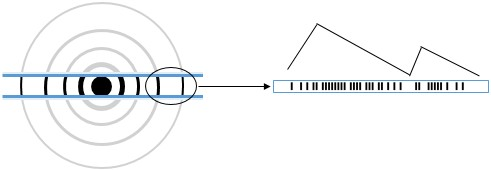
\includegraphics[scale=1]{sections/images/consciousness_waves.jpg}
	\floatfoot{Padrão de onda inferido pela tendência dessa distribuição com frequências maiores sentido a mediana da população e a baixíssima probabilidade de crescimento uniforme dessas frequências.}%\footnotemark}
	\end{figure}
	%\footnotetext{Fonte: note}

A junção de duas ondas além de eliminar suas discrepâncias, faz com que a primeira onda da união fique maior e a segunda onda acabe por deixar de existir a se tornar parte da primeira, que tem seu pico mais próximo da mediana. Probabilisticamente uma onda não morre, apenas une-se com outras ondas mais centrais a ela.
	\begin{figure}[H]
	\caption{Unificação de ondas}
	\label{fig:consciousness_uniform_wave}
	\centering
	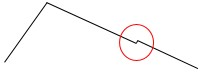
\includegraphics[scale=1]{sections/images/consciousness_uniform_wave.jpg}
	\floatfoot{Ondas sendo unificadas para exemplificar o crescimento amostral uniforme.}%\footnotemark}
	\end{figure}
	%\footnotetext{Fonte: note}

\subsubsubsection{Entrelaçamento e subconsciente}
As amostras que mais se parecem em termos de frequências e distribuição são as amostras que fazem parte da mesma onda. Elas são frequências opostas não sobrepostas que se completam.

Probabilisticamente as duas partes complementares de uma onda estarão a uma distância aproximadamente iguais, equidistante da mediana, porém essa não é uma regra e as partes complementares de uma onda podem estar em distâncias diferentes da mediana. O fenômeno da paridade das partes de uma onda tem o nome de entrelaçamento de ondas.

Essas ondas formam subconsciências de uma consciência maior. A consciência é única para todo o intervalo, é a lógica do intervalo, enquanto formam subconsciências, como pequenas ondas de uma onda maior. Assim, uma mudança na onda maior (consciência) também é uma mudança na onda menor (subconsciência), mudança essa que é induzida pelas subconsciências indiretamente, análogo ao comprimir gás em um cilindro, onde ao adicionar uma nova molécula de gás no cilindro parcialmente cheio, mais próximas ou apertas as moléculas dentro dele estarão. O contrário também é verdadeiro, uma nova amostra em uma subconsciência que por esta é observada diretamente é também uma mudança da consciência e vai ser induzida por outras subconsciências indiretamente.
	\begin{figure}[H]
	\caption{Subconsciência}
	\label{fig:consciousness_subconscious}
	\centering
	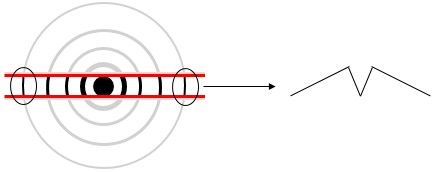
\includegraphics[scale=1]{sections/images/consciousness_subconscious.jpg}
	\floatfoot{O padrão de ondas forma subconsciências semelhantes ao padrão criado pela consciência (histograma de distribuição normal) como visto na Figura \ref{fig:statisticsbyjim_central_limit_theorem} ou na Figura \ref{fig:trend_chart_of_normal_distribution}.}%\footnotemark}
	\end{figure}
	%\footnotetext{Fonte: note}

\subsubsubsection{Salto}
O salto é uma reordenação feita pelo entrelaçamento de ondas a medida que as amostras do entrelaçamento deixam de ser equivalentes com a adição de novas amostras em seus lados.

Na Figura \ref{fig:consciousness_space_subconscious_observation_jump} é observado os entrelaçamento de ondas (representadas por colunas do histograma na vertical). A reordenação feita pelo entrelaçamento provoca um salto nas coordenadas (X, Y e Z) conforme subseção do Espaço.
	\begin{figure}[H]
	\caption{Reordenação subconsciente - Salto}
	\label{fig:consciousness_space_subconscious_observation_jump}
	\centering
	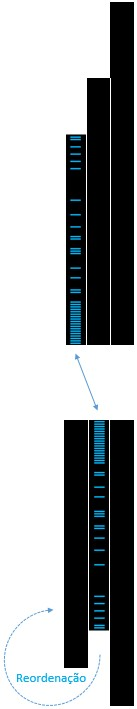
\includegraphics[scale=.6]{sections/images/consciousness_space_subconscious_observation_jump.jpg}
	\floatfoot{Salto provocado pela não equivalência do entrelaçamento com a adição de novas amostras.}%\footnotemark}
	\end{figure}
	%\footnotetext{Fonte: note}

A tendência probabilística é que, por exemplo, o elétron que saltou de sua orbita de origem retorne à esta conforme mais amostras são adicionadas ao entrelaçamento desse átomo, estabelecendo a normalidade probabilística.

\subsubsection{Tempo}
O tempo é a adição de novos momento lógicos entre momentos existentes à medida que prossegue a negação de si da lógica. Essas mudanças são acumulativas e a medida que aumentam o número desses momentos lógicos, menos relevante cada novo momento será dentro do intervalo consciente. Um em cem é mais relevante do que um em mil. 
	\begin{figure}[H]
	\caption{Tempo}
	\label{fig:consciousness_time}
	\centering
	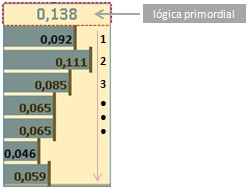
\includegraphics[scale=.8]{sections/images/consciousness_time.jpg}
	\floatfoot{Progressão do tempo conforme os momentos lógicos avançam.}%\footnotemark}
	\end{figure}
	%\footnotetext{Fonte: note}

Outro fator importante a observar do tempo é que, probabilisticamente, subconsciências mais próximas da mediana da população terão uma adição maior de novas amostras em seus intervalos, o que são observados diretamente por essas subconsciências. Por outro lado, subconsciências distantes da mediana da população terão uma adição menor de amostras em seus intervalos e sujeitam-se a um número maior de mudança induzidas indiretamente. Esse fenômeno de observação temporal proporcionado pela consciência e subconsciências evita o paradoxo dos gêmeos \cite{brasilescola_paradoxo_gemeos}.

Na seção Expansão lógica foi apresentado que a lógica é uma sequência de negações de si no tempo zero, ou seja, em nenhum momento entre suas negações a lógica passa a SER, garantindo a premissa primordial da constante lógica, NÃO SER. Assim, a lógica é uma sequência infinita e simultânea, uma constante. Logo, o tempo é apenas uma grandeza da consciência oriunda da ordenação dessa sequência lógica, não da sequência propriamente. A simultaneidade dessa sequência torna a lógica uma constante com todas as suas infinitas possibilidades, sendo esse universo uma delas. 

Cada universo tem uma ordem diferente em sua sequência e é essa ordem que dá origem à grandeza que chamamos de tempo. É essa ordem do universo ou consciência que vai dar a noção do que acontece antes ou depois, ou seja, o passado, o presente e o futuro. 

Na experiência do tempo conduzida pela consciência a ordenação da sequência é a essência dessa grandeza e, portanto, mais relevante do que sua origem que é de natureza simultânea.

\subsubsection{Espaço}
As ondas da consciência exibidas em forma de histograma, onde as partes das ondas que se completam são colocados lado a lodo é exibida na Figura \ref{fig:consciousness_space_waves}. A formação desse histograma é proveniente do entrelaçamento de ondas.
	\begin{figure}[H]
	\caption{Histograma proveniente do entrelaçamento de ondas}
	\label{fig:consciousness_space_waves}
	\centering
	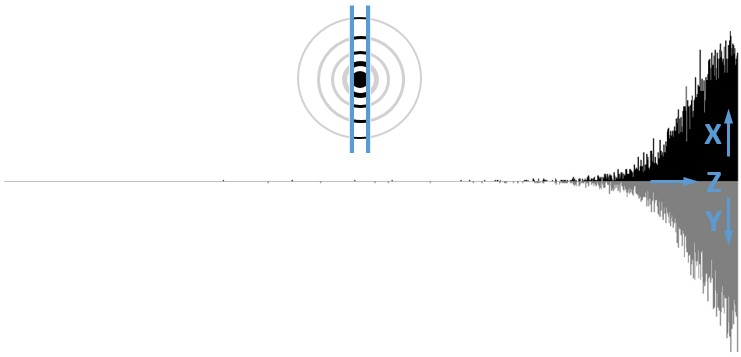
\includegraphics[scale=.7]{sections/images/consciousness_space_waves.jpg}
	\floatfoot{Exemplo do padrão de ondas obtido pelo algoritmo Logic\_WavePattern. \footnotemark}
	\end{figure}
	\footnotetext{O algoritmo Logic\_WavePattern pode ser visto no Apêndice \ref{app:algoritmos}.}

Ao representar as grandezas espaciais do gráfico da Figura \ref{fig:consciousness_space_waves} em um gráfico de distribuição 3D e distribuir seus pontos de extremidade (desprezando seus volumes e possíveis pontos internos), obtém-se algo parecido com uma espiral (como redemoinhos no ar ou na água) mesmo em volumes muito pequenos de dados (poucos momentos lógicos), conforme Figuras \ref{fig:consciousness_space_3DScatter15000-10} e \ref{fig:consciousness_space_3DScatter_200000-2}. Os pontos se movem em formato de espiral, aproximadamente, uma vez que as coordenadas X, Y e Z aumentam à medida que novas amostras são adicionadas na população.
	\begin{figure}[H]
	\centering
		\begin{subfigure}[H]{0.47\linewidth}
		\centering
		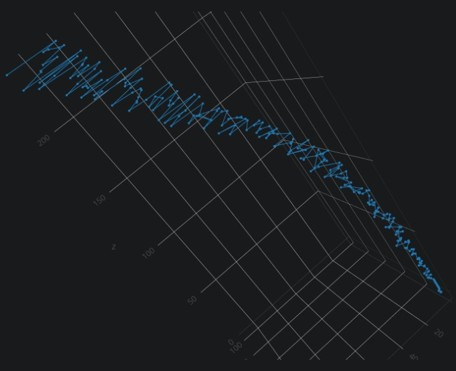
\includegraphics[width=.96\linewidth]{sections/images/consciousness_space_3DScatter15000-10.jpg}
		\caption{15.000 amostras ou momentos}
		\label{fig:consciousness_space_3DScatter15000-10}
		\end{subfigure}
	\hfill
		\begin{subfigure}[H]{0.47\linewidth}
		\centering
		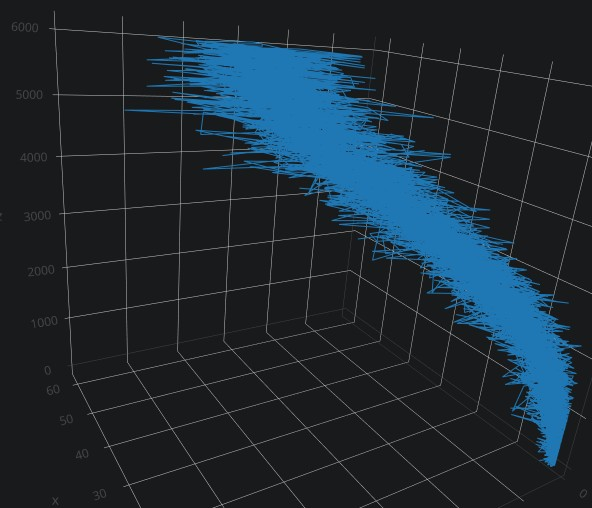
\includegraphics[width=.9\linewidth]{sections/images/consciousness_space_3DScatter_200000-2.jpg}
		\caption{200.000 amostras ou momentos}
		\label{fig:consciousness_space_3DScatter_200000-2}
		\end{subfigure}%
	\caption{Gráfico de dispersão 3D gerado com os pontos da Figura \ref{fig:consciousness_space_waves}}
	\floatfoot{O histograma no padrão de ondas e os dados para gerar o gráfico de dispersão 3D podem ser obtidos com a execução do algoritimo Logic\_WavePattern. \protect\footnotemark}
	\end{figure}
	\footnotetext{O algoritmo Logic\_WavePattern pode ser visto no Apêndice \ref{app:algoritmos} e os gráficos de dispersão 3D podem ser acessados em: \url{https://chart-studio.plot.ly/create/?fid=ren.stuchi:5&fid=ren.stuchi:4} e \url{https://chart-studio.plot.ly/create/?fid=ren.stuchi:7&fid=ren.stuchi:6}}

\subsubsubsection{Intervalos}
A observação de outras subconsciências depende do range de ondas que uma subconsciência é capaz de observar e esse range, por sua vez depende do range de ondas que a própria subconsciência é constituída. Todos os possíveis intervalos que se correspondem em X e Y encontram-se simultaneamente formando ondas em diferentes níveis.

Em ranges de muitos momentos lógicos pode-se ver o agrupamento de grandes objetos (subconsciências), sendo o maior deles representado pela cor azul claro e os menores e mais distantes pela cor azul escuro ou roxo, conforme Figura \ref{fig:consciousness_space_subconsciousness}. Esse agrupamento pode representar, por exemplo, o centro do universo, então o centro de uma galáxia, estrelas, planetas e objetos menores e mais distantes.
	\begin{figure}[H]
	\caption{Abstração espacial das subconsciências - grandes agrupamentos}
	\label{fig:consciousness_space_subconsciousness}
	\centering
	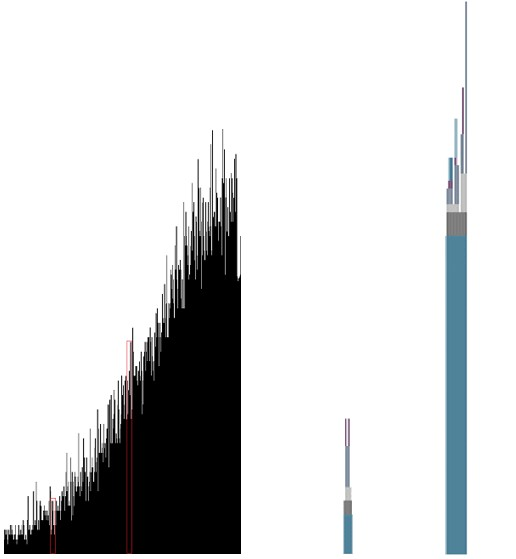
\includegraphics[scale=.5]{sections/images/consciousness_space_subconsciousness.jpg}
	\floatfoot{Caracteristicas da ondas formadoras da subconsciência de grandes objetos.}%\footnotemark}
	\end{figure}
	%\footnotetext{Fonte: note}

Em ranges com uma quantidade menor de momentos lógicos pode-se ver o agrupamento de pequenos objetos (subconsciências). Quanto menores os agrupamentos menos divisões esses agrupamentos têm (cores) e mais estreitos e compridos eles são, conforme Figura \ref{fig:consciousness_space_subconsciousness_min}. Esse agrupamento pode representar, por exemplo, o átomo que são muito pequenos, se apresentam em enormes quantidades e as partículas que orbitam seu núcleo (elétrons) ficam bem mais distantes dele.
	\begin{figure}[H]
	\caption{Abstração espacial das subconsciências - pequenos agrupamentos}
	\label{fig:consciousness_space_subconsciousness_min}
	\centering
	
\includegraphics[scale=.7]{sections/images/consciousness_space_subconsciousness_min.jpg}
	\floatfoot{Caracteristicas da ondas formadoras da subconsciência de pequenas partículas.}%\footnotemark}
	\end{figure}
	%\footnotetext{Fonte: note}}
	
As cores dos agrupamentos indicam a relação entre conjuntos e subconjuntos. Subconjuntos nascem de conjuntos ou outros subconjuntos e essa relação paterna filial é permanente. Conjuntos e subconjuntos também podem se dividir no mesmo nível, a depender do entrelaçamento das amostras.

\subsubsubsection{Volume}
O volume dobra a cada um terço de crescimento das amostras ou momentos lógicos de um agrupamento, aproximadamente. Como exibido na Figura \ref{fig:consciousness_space_volume}, os momentos lógicos ficam mais concentrados no começo das ondas entrelaçadas, o que pode gerar algo de fácil observação nessa região, como estrelas, planetas etc. 
\begin{figure}[H]
	\caption{Amostras vs volume}
	\label{fig:consciousness_space_volume}
	\centering
	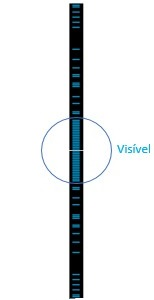
\includegraphics[scale=.8]{sections/images/consciousness_dark_matter_dark_energy_wave.jpg}
	\floatfoot{O volume em três dimensões dobra a cada um terço de crescimento das amostras, aproximadamente.}%\footnotemark}
	\end{figure}
	%\footnotetext{Fonte: note}}

\subsubsubsection{Espiral}
Os subconjuntos de um agrupamento tendem a formar espirais em seus movimentos que podem ser melhor entendidas e observadas na Figura \ref{fig:consciousness_space_spiral}.

Cada agrupamento tem sua própria linha de referência. Assim como dentro de um metro existem os centímetros, milímetros etc., dentro de um agrupamento existem outros agrupamentos.
	\begin{figure}[H]
	\caption{Detalhes do movimento em espiral}
	\label{fig:consciousness_space_spiral}
	\centering
	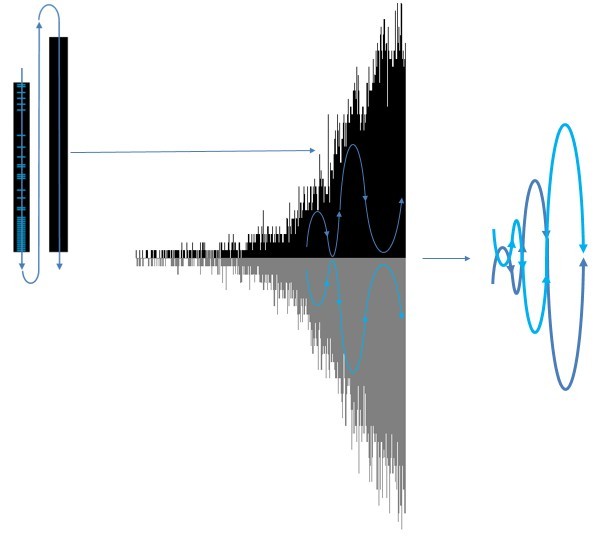
\includegraphics[scale=.8]{sections/images/consciousness_space_spiral.jpg}
	\floatfoot{Detalhes do movimento em espiral dos subconjuntos de amostras.}%\footnotemark}
	\end{figure}
	%\footnotetext{Fonte: note}}

Na Figura \ref{fig:consciousness_space_spiral} foi refletida as amostras da linha de referência para os eixos X e Z para facilitar as observações. As observações abaixo relacionadas ao eixo X também se aplicam ao eixo Y:
	\begin{description}
	   \item[Linha de referência] Representa uma diagonal entre os eixos X, Y e Z onde os subconjuntos (traços como representados no exemplo de A e B) estão dispostos ao redor dessa linha e se afastando dela à medida que os valores das coordenadas aumentam.
	   \item[A e B] Os traços representados no exemplo de A e B são subconjuntos de uma população. Quando mais amostras em um subconjunto mais estável e harmônicos são seus movimentos espirais probabilísticos em torno de sua linha de referência. Os subconjuntos em A representam a média mínima probabilística de X para esse intervalo Z. Já os subconjuntos em B representam a média máxima probabilística de X para esse intervalo Z. Visto que os subconjuntos se dispõem probabilisticamente ao redor da linha de referência, então os subconjuntos e A por estarem na média mínima tendem probabilisticamente a receber mais amostras que os subconjuntos em B, fazendo com que os subconjuntos em A se elevem em X mais rapidamente que os subconjuntos em B que por estarem recebendo menos amostras, nesse cenário, passam a estar em uma elevação de X menor.
	   \item[X1 e X2] A adição de novas amostras à população formam novos subconjuntos antes e depois dos representados por A e B. Assim, as coordenadas X, Y e Z de A e B aumentam e faz com que esses se movimentem a frente, como exemplificado por B. É importante notar que os subconjuntos em B mesmo com uma elevação probabilística em X menor continuam a aumentar o valor de X mesmo com a impressão de que o valor X diminuiu, conforme mostrado por X1 e X2.
	\end{description}

Na Figura \ref{fig:consciousness_space_spiral_direction} é exibida a orientação da parte visível de um objeto juntamente com o espaço que completa a formação deste objeto.
	\begin{figure}[H]
	\caption{Orientação do movimento em espiral}
	\label{fig:consciousness_space_spiral_direction}
	\centering
	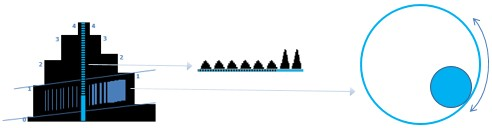
\includegraphics[scale=1]{sections/images/consciousness_space_spiral_direction.jpg}
	\floatfoot{Detalhes do orientação do movimento em espiral dos subconjuntos de amostras.}%\footnotemark}
	\end{figure}
	%\footnotetext{Fonte: note}}
	
\subsubsection{Forças fundamentais}
A força gravitacional, a força eletromagnética e a força nuclear correspondem às forças fundamentais da natureza e essas forças também são provenientes do entrelaçamento de ondas, como o espaço. As forças fundamentais não são forças propriamente, mas sim aspectos probabilísticos (distribuição normal) e do entrelaçamento de ondas principalmente.

\subsubsubsection{Força gravitacional}
O entrelaçamento ondas é o aspecto que coordena as mudanças nas coordenadas espaciais junto com a adição de novos momentos lógicos sentido a mediana da população. As mudanças dessas coordenadas provocam iterações que podem ser vistas nas Figuras \ref{fig:consciousness_space_3DScatter15000-10} e \ref{fig:consciousness_space_3DScatter_200000-2} da subseção de Espaço e na Figura \ref{fig:consciousness_dark_matter_dark_energy_wave} que mostra probabilisticamente onde está a maior concentração de momentos lógicos de um intervalo consciente ou subconsciente, devido a estes momentos serem mais intensos sentido a mediana. Estes aspectos são chamadas de gravidade.

\subsubsubsection{Força eletromagnética}
A força eletromagnética é uma especificação do aspecto gravitacional que depende da aproximação espacial (redução de diferenças nos eixos X, Y e Z) e do entrelaçamento de ondas.

Quando um objeto se aproxima de outro, seus pares de ondas provenientes do entrelaçamento de ondas ficam cada vez mais parecidos, eixos X e Y. Essa proximidade faz com que as partes das ondas de um objeto se pareça muito com as partes das ondas do outro objeto, o que pode fazer com que o entrelaçamento de ondas encontre pares mais ideais nesse outro objeto e vice-versa.  

As linhas azuis da Figura \ref{fig:consciousness_electromaagnetic_force} mostra onde é mais frequente a troca dos pares de ondas pelo entrelaçamento de ondas, ou seja, onde se tem a maior probabilidade das ondas serem parecidas. Por isso os imãs tentam se virar para se conectar quando estão face a face com o mesmo polo. As linhas cinza mostram as conexões que ocorrem em número bem menor. 
	\begin{figure}[H]
	\caption{Força eletromagnética}
	\label{fig:consciousness_electromaagnetic_force}
	\centering
	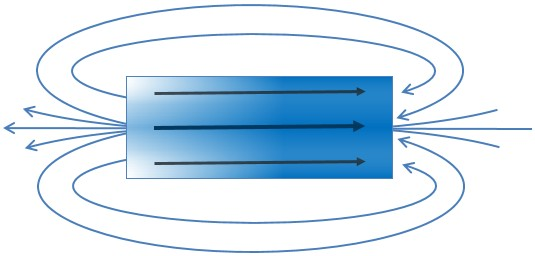
\includegraphics[scale=.6]{sections/images/consciousness_electromaagnetic_force.jpg}
	\floatfoot{Aumento das possibilidades de entrelaçamento de ondas devida a aproximação e o menor número de momentos lógicos das menores partículas. }%\footnotemark}
	\end{figure}
	%\footnotetext{Fonte: note}

Com a troca de significativos pares de ondas entre os objetos faz-se a mixagem do posicionamento dos eixos X, Y e Z entre esses objetos ocorrendo a aproximação deles no espaço. 

Quanto menor a partícula (elétron ou partículas menores), conforme Figura \ref{fig:consciousness_space_subconsciousness_min}, mais fácil o entrelaçamento ocorre. Provavelmente muitos objetos não tenham alta capacidade de entrelaçamento devido aos seus elétrons ou partículas menores serem formadas por muitos momentos lógicos (barras do histograma mais largas ou mais compridas), ou seja, quanto maior a quantidade de momentos dessas partículas menores as chances de entrelaçamento.

Probabilisticamente as partículas mais parecidas estão nas regiões mais próximas (linhas azuis do Figura \ref{fig:consciousness_electromaagnetic_force}) devido ao crescimento do número de amostras sentido a mediana da população, porém isso não é uma regra e os polos podem se inverter, ou seja, ter mais ligações com a região de menor probabilidade (isso não quer dizer que houve formação de antimatéria nessa região, as partículas ainda tendem a concentrar mais momentos lógicos sentido à mediana da população). No entanto, a probabilidade tende a corrigir esses polos conforme novos momentos vão sendo adicionadas nesse intervalo.

\subsubsubsection{força nuclear}
As forças nucleares forte e fraca representam as maiores concentrações de momentos lógicos por intervalo populacional. Esses picos podem ser vistos na Figura \ref{fig:consciousness_space_subconsciousness_min} e eles não param de crescer à medida que novos momentos lógicos são adicionados nestes intervalos. Estes momentos ou amostras tendem a estarem cada vez mais juntos dentro do intervalo formando picos cada vez mais altos.

\subsubsection{Matéria escura e energia escura}
Quanto maior o número de amostras e mais próximas elas estão da mediana, mais elas farão parte dos 99,99\% e ainda mais amostras também estarão nos 0,01\%, conforme a Tabela \ref{tab:10000_all}. Logo, a energia escura não é uma energia propriamente, mas sim um aspecto probabilístico. 
	\begin{figure}[H]
	\caption{Aspecto probabilístico da energia escura}
	\label{fig:consciousness_dark_matter_dark_energy}
	\centering
	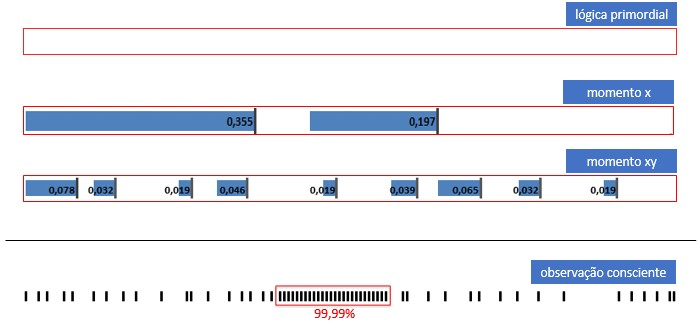
\includegraphics[scale=1]{sections/images/consciousness_dark_matter_dark_energy.jpg}
	\floatfoot{A energia escura não é uma energia propriamente, mas sim um aspecto probabilístico.}%\footnotemark}
	\end{figure}
	%\footnotetext{Fonte: note}

Já a matéria escura, como pode ser visto na Figura \ref{fig:consciousness_dark_matter_dark_energy_wave} mostra probabilisticamente onde está a maior concentração das amostras de um intervalo, tornando mais fácil a visualização por outras subconsciências, uma vez também que o volume dobra a cada um terço do crescimento das colunas do histograma, aproximadamente, conforme dito na seção do Espaço. Assim, uma grande área do intervalo de um agrupamento pode conter amostras dispersas que se tornam mais difíceis de observar. O aspecto descrito acima e demostrado pela Figura \ref{fig:consciousness_dark_matter_dark_energy_wave} é aplicável a qualquer intervalo de um agrupamento (Figuras \ref{fig:consciousness_space_subconsciousness} e \ref{fig:consciousness_space_subconsciousness_min}).
	\begin{figure}[H]
	\caption{Analogia da matéria escura}
	\label{fig:consciousness_dark_matter_dark_energy_wave}
	\centering
	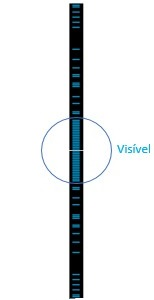
\includegraphics[scale=.9]{sections/images/consciousness_dark_matter_dark_energy_wave.jpg}
	\floatfoot{Parte do volume é facilmente observado por outras subconsciências.}%\footnotemark}
	\end{figure}
	%\footnotetext{Fonte: note}

\subsubsection{Antimatéria}
Independente do intervalo observado, sua maior concentração de amostras tende a estar sentido da mediana, o que é o sentido provável conforme teorema central do limite. Essas amostras também podem estar com sua concentração no sentido oposto à mediana, porém com uma ocorrência probabilística cada vez menos conforme as amostras aumentam. Na Figura \ref{fig:consciousness_concentration_of_opposite_samples} é exibido dois intervalos idênticos com suas amostras com concentrações opostas.
	\begin{figure}[H]
	\caption{Parte de um intervalo idêntico com suas concentrações de amostras opostas}
	\label{fig:consciousness_concentration_of_opposite_samples}
	\centering
	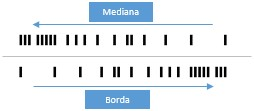
\includegraphics[scale=1]{sections/images/consciousness_concentration_of_opposite_samples.jpg}
	\floatfoot{Parte de um intervalo idêntico distribuídos de formas opostas.}%\footnotemark}
	\end{figure}
	%\footnotetext{Fonte: note}

O merge ou soma dos intervalos opostos da Figura \ref{fig:consciousness_concentration_of_opposite_samples} os tornaria um intervalo simétrico, ou seja, não estaria em nenhum dos sentidos.
Na Figura \ref{fig:consciousness_concentration_of_opposite_samples_within_range} é exibido um intervalo consciente completo com suas concentrações de amostras sentido à mediana e outro idêntico, mas com suas concentrações sentido às bordas do intervalo.
	\begin{figure}[H]
	\caption{Intervalos conscientes com suas concentrações de amostras opostas}
	\label{fig:consciousness_concentration_of_opposite_samples_within_range}
	\centering
	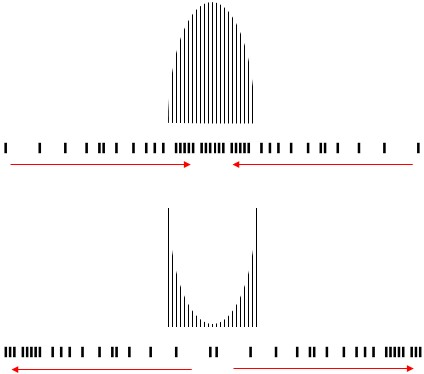
\includegraphics[scale=.8]{sections/images/consciousness_concentration_of_opposite_samples_within_range.jpg}
	\floatfoot{Intervalos conscientes completos e idênticos distribuídos de formas opostas.}%\footnotemark}
	\end{figure}
	%\footnotetext{Fonte: note}


\subsubsection{Buraco negro}
O buraco negro é uma concentração muito alta de amostras, formada por grandes agrupamentos subconscientes, Figura \ref{fig:consciousness_space_subconsciousness}.
Esses grandes agrupamentos ocupam grandes volumes de espaço devido a quantidade de amostras. 

Os grandes volumes são encontrados na base dos grandes agrupamentos, conforme as cores azul claro e cinza da Figura \ref{fig:consciousness_black_hole}.
	\begin{figure}[H]
	\caption{Buracos negros}
	\label{fig:consciousness_black_hole}
	\centering
	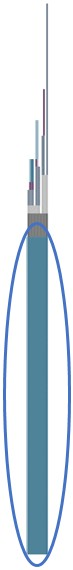
\includegraphics[scale=.6]{sections/images/consciousness_black_hole.jpg}
	\floatfoot{Grandes volumes são encontrados na base dos grandes agrupamentos.}%\footnotemark}
	\end{figure}
	%\footnotetext{Fonte: note}

% ----------------------------------------------------------
% Subseção Observações
% ----------------------------------------------------------
\subsection{Observações}

\begin{description}
   \item[Rigidez lógica] Se a rigidez física e suas leis parecem ser intransponíveis, abaixo dela está à lógica, ainda mais rígida e intransponível, pois fora da lógica o que se tem é o inexistente, o ilógico. A existência está contida nas possibilidades do que é lógico. 
   \item[Matemática] A matemática é uma ótima abstração do universo, mas ela não é a linguagem do universo, pois abaixo da matemática está à lógica, a base da matemática e de toda a existência.
   \item[Bem e mal] O bem e o mal são observações das subconsciências. Ou seja, se está claro a negação tende a escurecer, se está calor a esfriar etc. É a briga dos contrários de Heráclito de Éfeso.
   \item[Perfeição] A lógica primordial é a mais simples das lógicas, é a essência da existência. Uma lógica tão simples quanto eficiente, tão eficiente quanto perfeita. A lógica mais poderosa:
   \begin{description}
	   \item[Onipotente] A essência de todas as possibilidades lógicas, ou seja, a essência da existência, pois fora das possibilidades lógicas está o ilógico, o inexistente;
	   \item[Onisciente] Fluxo de todas as abstrações lógicas desde a consciência às subconsciências; 
	   \item[Onipresente] Suas frações (negações) estão em toda a existência.
   \end{description}
Essas observações remetem a Deus, a consciência das subconsciências.
   \item[Realidade] Como possibilidade lógica o sonho é tão real quando a "realidade". Talvez o estudo das possibilidades lógicas leve a caminhos onde os sonhos possam ser tão reais quanto à realidade, já que os dois não passam de lógica, como sonhos lúcidos, por exemplo \cite{ administradores_principio_pareto}. Isso talvez explique por que outras possíveis formas de vidas "inteligentes", quando evoluídas, deixam de buscar esse tipo de vida em um possível vasto universo à procurarem dentro de si, onde se pode encontrar algo bem maior que o universo, o infinito.
\end{description}